\chapter{Connecting The Dots...}
While the concepts mentioned in the previous chapter might seem disparate at first, they are closely related with one other and each of them follows naturally from the preceding one. This chapter is aimed at eliciting the flow between these topics. 

While the background theme of the project is deployable structures, this gradually diverged to encompass several ideas mentioned in the first chapter.

\section{Deployable Structures and Mechanisms}
As mentioned earlier, there are two approaches taken for development of deployable structure, namely structural components and generative techniques. The concepts of mechanisms come in the picture through the first way. 

While the Maxwell's rule provides condition for the static and kinematic determinacy based on the equality of number of equations and number of unknowns when structure is adequately connected to the foundation as 
\begin{equation}
    b = dJ,
\label{eq:cacona}
\end{equation}

\noindent where b is the total number of bars, d is dimension of the problem and J is the number of non foundation joints.

However, exceptions exist to this rule in form of structures which satisfy Maxwell's rule but still are kinematically indeterminate.

A more exhaustive treatment of equilibrium and kinematic matrix provides a more complete explanation for these anomalies.

The equilibrium matrix of a structure is a $(3j - k)$ by $b$ matrix which relates the member tensions $\boldsymbol{t}$ with external loads $\boldsymbol{f}$ as
\begin{equation}
    \boldsymbol{A.t = f}
    \label{eq:cacona}
\end{equation}
\noindent where j is total number of joints, k is number of kinematic constraint on foundation joints and b is the total number of bars.

In a similar manner, for small deformations, member elongations $\boldsymbol{e}$ and displacements of joints $\boldsymbol{d}$ can be related using a $b$ by $(3j - k)$ matrix $\boldsymbol{B}$ as
\begin{equation}
    \boldsymbol{B.d = e}
    \label{eq:cacona}
\end{equation}

\noindent Using the principle of virtual work, one can show that $\boldsymbol{B = A^T}$. The fundamental sub-spaces associated with these matrices and there significance are as following:

\begin{enumerate}
    \item \textit{Column Space of A} : Provides the range of $\boldsymbol{f}$ that can be supported by the structure and modes of displacement that require elongation of one or more bars.

    \item\textit{Left nullspace of A} : Describes the range of $\boldsymbol{f}$ that can not be supported by the structure in its original configuration and it is the space spanned by inextensional mechanisms.

    \item\textit{Row Space of A} : Spans the space generated by bar tensions in equilibrium with the applied load and describes geometrically compatible bar elongations.

    \item\textit{Nullspace of A} : represents sets of tension which are in equilibrium with zero loads (states of self stress) and bar elongations forbidden by the geometry.
\end{enumerate}



The analysis of these sub-spaces associated with the matrices $\boldsymbol{A}$ and $\boldsymbol{B}$ results in modified Maxwell's equation as
\begin{equation}
    s = b - r_{A},  \hspace{1cm} m = 3j - k - r_{A},
    \label{eq:cacona}
\end{equation}
\noindent subtracting two equations we get
\begin{equation}
    s - m = b - 3j + k
    \label{eq:cacona}
\end{equation}
\noindent here s is the number of states of self stress, and m is the number of mechanisms present in the structure. $r_{A}$ is the rank of the matrix A.

Further investigation of these matrices provides us with a way to distinguish between finite and infinitesimal mechanisms. These insights coupled with the interpretation of fundamental sub-spaces provide the information necessary for design of mechanism based deployable structures\cite{Pelle}. 

\section{Deployable Structures and Origami}
Origami aids in the development of deployable structures through the generative pathway\cite{rivas2015deployable}. Origami provides a way to pack the structures into compact spaces. Today, applications of origami and paper fold concepts are widely used in aerospace applications. The origami models can be morphed into real structure by developing the equivalent bar and hinge models\cite{FilipBarandHinge}. The simplicity of such models make them well suited for the origami engineering community, and their efficiency make them suitable for design problems such as optimization and parameterization of geometric origami variations.The application of origami for development of deployable structures can be best illustrated by examples as shown in the Fig~\ref{fig:OrigamiEx}.
\begin{figure}[htbp]
    \centering
    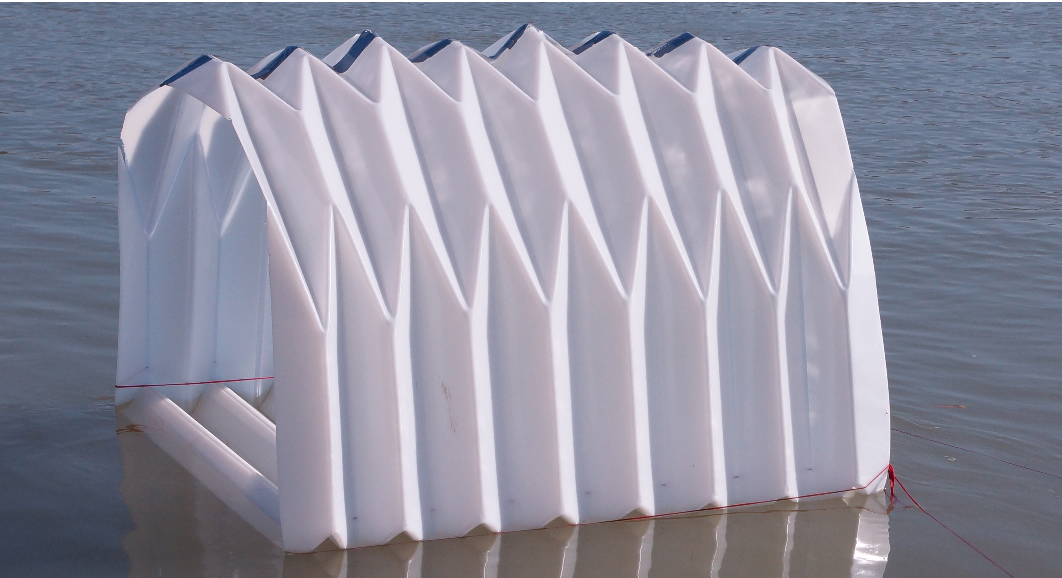
\includegraphics[width = 0.5\linewidth]{introduction/fig/OrigamiEx.png}
    \caption{Origami for disaster relief structure \cite{Tepa}}
    \label{fig:OrigamiEx}
\end{figure}


Furthermore the concepts of origami combined with the metamaterials provide a way for the structures which follow different energy pathways during deployment and contraction, which makes them highly desirable since they can be designed to resist immediate collapse by providing an energy barrier in their contraction pathway\cite{Zha}. This also adds to the reliability for use of deployable structures making their stability less dependent on locking mechanisms. In addition to this Origami can also be used for programming curvatures\cite{Dud}, and development of metamaterials\cite{Filip}.

In simple cases of pure origami based deployable hollow triangulated cylinders, based on the energy required the structures can be classified as easy-deploy-easy-collapse (requiring no or minimal energy for deployment as well as collapse) or hard-deploy-hard-collapse (requiring significant amount of energy for deployment as well as collapse). Easy-deploy-easy-collapse structures generate minimal strain in members of their equivalent bar and hinge model while hard-deploy-hard-collapse structure create large strains leading to even failure in case of conventional materials\cite{Zha,FilipBarandHinge}. The tubes can be designed to fall in one of the types by varying simple parameters which is shown in the next chapter.

\section{Deployable Structures and Metamaterials}
The domain of metamaterials which deals with materials having tunable stiffness forms a connection between metamaterials and deployable structure. Simplest instance of use of metamaterials in deployables is in the structures which have different energy paths for deployment and collapse, as explained earlier. Using a conventional material, if an element experiences compression during the process of deployment, it will experience tension while collapsing and usually the stiffness in tension as well as compression is same for materials and thus energy path followed is same for two deployment as well as collapse, however for material which exhibit different stiffness for tension and compression will have different profiles for two process and can lead to structures which deploy easily but offer resistance for collapsing and vice versa.\cite{Zha} 

Furthermore soft metamaterials and materials at the verge of instability have parameters which can be tuned to develop hinges and joints as part of elements engendering the possibility of a unified deployable systems without any external joints.\cite{Baardink489, Rock}

Design of metamaterials also draws from Origami, Mechanism, Topology, and form finding making a cohesive whole of all these ideas\cite{Filip, Rock}.


\section{Deployable Structures and Form Finding}
The concepts of form finding approach the topic of deployable structure from other direction. The ideas of form finding are usually applied in the reverse direction to determine the boundary conditions which will lead to the structure taking the desired shape. The deformations involved are usually large and material needs to be elastic during the entire process so that the structure can be deployed and collapsed a number of times, this provides another entry point for the application of metamaterials.

An example where this relationship is elicited is that of form finding in elastic gridshells. Initially planar elastic grid is actuated into a shell like structure by loading their extremities. It was observed that the resulting shapes are complex even for simple configuration and indicated the presence of multi-stable states and higher order modes in the actuated grid. However it is possible to parameterize these complex shape and by varying these parameters desired actuated shape can be obtained\cite{Baek75}.

\section{Deployable Structures and Elastic Bilayers}
In general nonuniform in-plane growth of thin sheets results in out of plane buckling. This process is responsible for several process in nature such as shaping of leaf and blooming of flowers. Generally, such sheets settle in residually strained configuration which is a local minima of the energetic cost of stretching and bending the sheet. Since it's a local minima, this state might not be unique. By solving the inverse problem one can design the layer such that it can be used to achieve any target surface shape from any reference shape\cite{va}. Similar to the case of form finding, this involves parameterizing the surface and solving the inverse problem.

\section{Deployable Structures and Topological Mechanics}
Topology involves the study of connectivity of different elements in a system and is essential to the idea of deployable structures. Topology plays an important role in determining the member connectivity in deployable trusses and folding motions of Origami and Kirigami\cite{Che}.

In addition to the deployable structures, It has a huge role in development of metamaterial\cite{Rock, Berto, Surj} and lattice mechanics\cite{Ma}. Topology can be used to control the mechanical properties of a material along an edge or around a localized defect, topological polarization of a network governs along with its variation and orientation define the rigidity of the network. The topology of the lattices can be varied to move between states with dramatically varying mechanical properties such as elastic modulus, wave characteristics and so on. 

\section{Deployable Structures and Lattices}
The deployable structure connects with the lattices at two level, on a trivial level, the lattices can be considered as a special kind of structure and mechanisms involved in such structures connect them directly with the ideas of deployable structure. Lattices require special attention owing to their periodic boundary conditions. Depending on the topology of lattice, actuation may propagate throughout the lattice or may cease within a few unit cells \cite{Neli}. Furthermore, it can be shown that static determinacy and kinematic determinacy can not exist in these structures concurrently \cite{Gues}. 

On a more elaborate level, Metamaterials connect the deployable structures with lattices since design of metamaterials requires realization and application of lattice mechanics and properties which is ultimately utilized for development of deployable structures. Lattice mechanics is essential to the development of metamaterials with unusual elastic modulus and phonon gaps.\cite{Ma}